\chapter{Chapter 2 Design and Implementation}

% \begin{chapterabstract}
%     Use the chapterabstract environment, not the abstract environment, if you want to plant an abstract at the top of the chapter.
% \end{chapterabstract}


% \begin{quote}
% If needed Here's a quote environment.
% \end{quote}


% Here's a citation, so we don't get a "no citation warning" \cite{GolV13}. Here's a figure.
% \begin{figure}
%     \begin{centering}
%         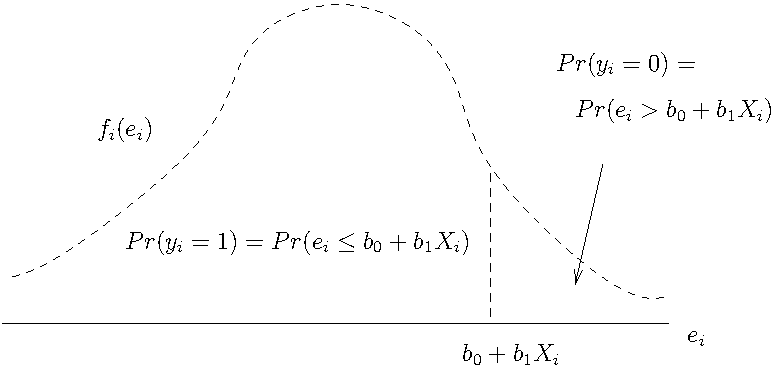
\includegraphics[scale=0.8]{design/chap_1_figures/example_1.pdf}
%     \par\end{centering}
%     \caption{Figure for list of figures  in the content page.}
%     \label{fig:first_fig}
% \end{figure}
% Here how to reference a figure such as Figure \ref{fig:first_fig}.
% \newpage

% \includestandalone[width=.8\textwidth]{chap_1_figures/State}

\section{Smart Contract Object Model}





\begin{table}

    \centering                       % Center your table

	\begin{tblr}{hlines, vlines}     % Your table
		Object Type & Action & C1  \\
		Collections & B2 & C2  \\
		A3 & B3 & C3
	\end{tblr}

	\caption{Operations}           % Caption
	\label{tab:my-first-table}       % Label
\end{table}
